% ================================= chapter 2 ================================= %
\chapter{モデリング}
\label{chapter_modeling}
\section{数式モデル}
制御器の設計のため,倒立振子系の状態方程式,観測方程式から数式モデルを導出する.

\subsection{状態方程式}

\begin{figure}[htbp]
    \begin{center}
        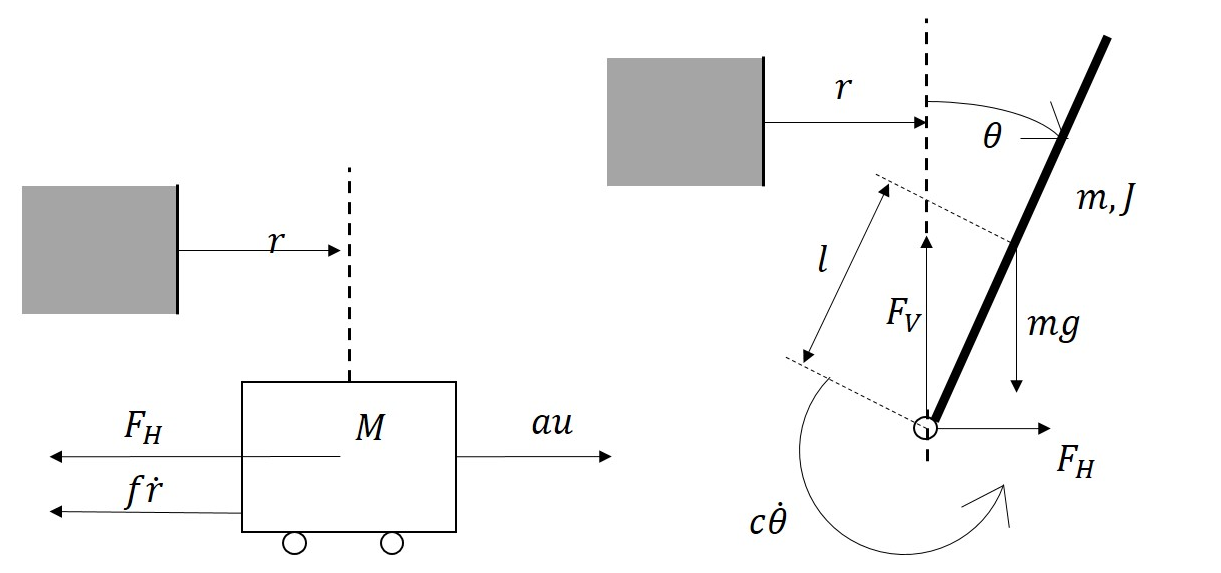
\includegraphics[width=0.6\linewidth]{modeling.eps}
        \caption{図\ref{modeling}: モデリングのための力の分解}
        \label{modeling}
    \end{center}
\end{figure}

図\ref{modeling}から導出した倒立振子系の運動方程式を
式(\ref{modeling:cart1})から式(\ref{modeling:pend2})に示す.

\begin{equation}
    M \ddot{r} = au - F_{H} - f \dot{r}
    \label{modeling:cart1}
\end{equation}
\begin{equation}
    J \ddot{\theta} = lF_{V}\sin{\theta} - lF_{H}\cos{\theta} - c \dot{\theta}
    \label{modeling:pend1}
\end{equation}
\begin{equation}
    m\frac{d^2}{dt^2}(r + l\sin{\theta}) = F_{H}
    \label{modeling:cart2}
\end{equation}
\begin{equation}
    m\frac{d^2}{dt^2}(l\cos{\theta}) = F_{V} - mg
    \label{modeling:pend2}
\end{equation}

ただし,$M$,$f$は台車の質量と摩擦係数,$m$,$l$,$c$,$J$は振子の質量,振子の重心から回転軸までの距離,
回転軸摩擦係数,重心周りに働く慣性モーメントである.また,$F_{H}$,$F_{V}$は振子が台車から受ける
水平効力と垂直抗力である.$F$はモータによる台車への駆動力であり,定数$a$,駆動アンプへの入力電圧$u$を用いて
式(\ref{F})で表される.

\begin{equation}
    F = au
    \label{F}
\end{equation}

ここで,系の状態$x$を4つの状態変数からなる縦ベクトルとする.すなわち,
$$
    x = \left[
    \begin{array}{c}
        r \\
        \theta \\
        \dot{r} \\
        \dot{\theta}
    \end{array}
    \right]
$$
と定義する.
次に,式(\ref{modeling:cart1})から式(\ref{modeling:pend2})から倒立振子系の非線形方程式を求める.
式(\ref{modeling:cart1}),式(\ref{modeling:pend1})から$F_{H}$を消去すると,式(\ref{del_Fh})が得られる.

\begin{equation}
    (M + m) \ddot{r} + (ml\cos{\theta}) \ddot{\theta} = au + (ml\sin{\theta}) \dot{\theta}^2 - f \dot{r}
    \label{del_Fh}
\end{equation}

また,式(\ref{modeling:pend1}),式(\ref{modeling:cart2}),式(\ref{modeling:pend2})から
$F_{H}$,$F_{V}$を消去すると,

$$
    J \ddot \theta = l\left(
        m\frac{d^2}{dt^2}\left(
            l\cos{\theta} + mg
            \right)
        \right)\sin{\theta}
        -
        l\left(
            m\frac{d^2}{dt^2}\left(
                r + l\sin{\theta}
            \right)
        \right)\cos{\theta}
$$

となり,式(\ref{del_Fh_Fv})が得られる.

\begin{equation}
    ml\cos{\theta} \ddot{r} + (J + ml^2) \ddot{\theta} = mgl\sin{\theta} -c \dot{\theta}
    \label{del_Fh_Fv}
\end{equation}

式(\ref{del_Fh}),式(\ref{del_Fh_Fv})を行列表現すると,

$$
    % --- left side --- %
    % --- Matrix first --- %
    \left[
    \begin{array}{cc}
        M + m          &  ml\cos{\theta} \\
        ml\cos{\theta}  &  J + ml^2
    \end{array}
    \right]
    % --- Matrix second --- %
    \left[
    \begin{array}{c}
        \ddot{r} \\
        \ddot{\theta}
    \end{array}    
    \right]
    =
    % --- right side --- %
    \left[
        \begin{array}{c}
            -f \dot{r} + ml(\sin{\theta)} \dot{\theta}^2 + au \\
            mgl\sin{\theta} - c \dot{\theta}
        \end{array}
    \right]
$$

$$
    % --- left side --- %
    \left[
    \begin{array}{c}
        \ddot{r} \\
        \ddot{\theta}
    \end{array}    
    \right]
    =
    % --- right side --- %
    % --- Matrix first --- %
    \left[
    \begin{array}{cc}
        M + m           &  ml\cos{\theta} \\
        ml\cos{\theta}  &  J + ml^2
    \end{array}
    \right]^{-1}
    % --- Matrix second --- %
    \left[
        \begin{array}{c}
            -f \dot{r} + ml(\sin{\theta)} \dot{\theta}^2 + au \\
            mgl\sin{\theta} - c \dot{\theta}
        \end{array}
    \right]
$$

となる.よって,

\begin{equation}
    \dot x = f(x, u) = 
    \left[
        \begin{array}{c}
            \dot{r} \\
            \dot{\theta} \\
            K^{-1}
            \left[
                \begin{array}{c}
                    -f \dot{r} + ml(\sin{\theta}) \dot{\theta}^2 + au \\
                    mgl\sin{\theta} - c \dot{\theta}
                \end{array}
            \right]
        \end{array}    
    \right],\
    K = 
    \left[
        \begin{array}{cc}
            M + m           &  ml\cos{\theta} \\
            ml\cos{\theta}  &  J + ml^2
        \end{array}
    \right]
    \label{nonlinear}
\end{equation}

が得られる.本実験では,不安定平衡点$x=0$近傍で線形化したモデルを採用できる.
$\theta$に関して式(\ref{nonlinear})を一次近似すると,
$\sin{\theta} \approx \theta,\ \cos{\theta} \approx 1,\ \theta^2 \approx 0$と近似できることから,

\begin{equation}
% --- Matrix x_dot --- %
    \dot x = 
    \left[
        \begin{array}{c}
            \dot{r} \\
            \dot{\theta} \\
            K^{-1}
            \left[
                \begin{array}{c}
                    -f \dot{r} + au \\
                    mgl \theta - c \dot{\theta}
                \end{array}
            \right]
        \end{array}    
    \right],\
    %--- Matrix K ---%
    K = 
    \left[
        \begin{array}{cc}
            M + m  &  ml \\
            ml     &  J + ml^2
        \end{array}
    \right]
    \label{linear_k}
\end{equation}

を得る.線形化された倒立振子系の状態方程式は,式(\ref{linear_general})のように表現される.

\begin{equation}
    \dot x = Ax + Bu
    \label{linear_general}
\end{equation}

ここで,

$$
    % --- Matrix A --- %
    A = 
    \left[
        \begin{array}{cc}
            O_{2 \times 2}  &  I_{2} \\
            A_{21}          &  A_{22}
        \end{array}
    \right],\
    % --- Matrix B --- %
    B = 
     \left[
        \begin{array}{c}
            O_{2 \times 1} \\
            B_{2}
        \end{array}
    \right]
$$

である.ただし,

$$
    A_{21} = K^{-1}
    \left[
        \begin{array}{cc}
            0  &  0 \\
            0  &  mgl
        \end{array}    
    \right],\
    A_{22} = K^{-1}
    \left[
        \begin{array}{cc}
            -f  &  0 \\
            0   &  -c
        \end{array}    
    \right],\
    B_{2} = K^{-1}
    \left[
        \begin{array}{c}
            a \\
            0
        \end{array}    
    \right]
$$

である.

\subsection{観測方程式}
2つの観測出力は,

$$
    y_{1} = c_{1} r
$$

$$
    y_{2} = c_{2} \theta
$$

のように表される.ここで,$c_{1}$は変位・電圧変換係数, $c_{2}$は角度・電圧変換係数である.
これらからなる縦ベクトル,すなわち出力$y$を,

$$
    y = 
    \left[
        \begin{array}{c}
            y_{1} \\
            y_{2}
        \end{array}    
    \right]
$$

と定義すると,倒立振子系に対する観測方程式を,

\begin{equation}
    y = Cx
\end{equation}

と表せる.ただし,

$$
    % --- Matrix N --- %
    N = 
    \left[
        \begin{array}{cc}
            c_{1}  &  0 \\
            0      &  c_{2}
        \end{array}
    \right],\
    % --- Matrix C --- %
    C = 
    \left[
        \begin{array}{cc}
            N  &  O_{2 \times 2}
        \end{array}
    \right]
    =
    \left[
        \begin{array}{cccc}
            c_{1}  &    0    &    0    &    0 \\
            0      &  c_{2}  &    0    &    0
        \end{array}
    \right]
$$

である.

\section{パラメータの同定}
パラメータの同定のため,以下の手順で測定を行う.

\begin{enumerate}
    \item 実測できるパラメータ$m$(振子の質量[kg]),$l$(振子の重心から回転軸までの長さ[m])の測定を行う.
    \item 駆動アンプへの入力電圧とモータ駆動力の変換係数$a$を求める.
    \begin{enumerate}
        \item 振子を台車から取り外す.
        \item モータに一定電圧$u$を加え,ばねばかりで引き,台車が正の方向に動き始めるときの力($au+$摩擦力)
        を$f_{max}$,負の方向に動き始めるときの力($au-$摩擦力)を$f_{min}$とする.測定は
        $10$[V], $11$[V], ..., $15$[V]の各電圧に対して行う.
        \item $f_{max}$, $f_{min}$それぞれの回帰直線の傾きを平均し,その値を$a$[N/V],
        すなわち入力電圧$u$[V]とモータ駆動力$f$[N]の変換係数とする.
        \begin{figure}[htbp]
            \begin{center}
                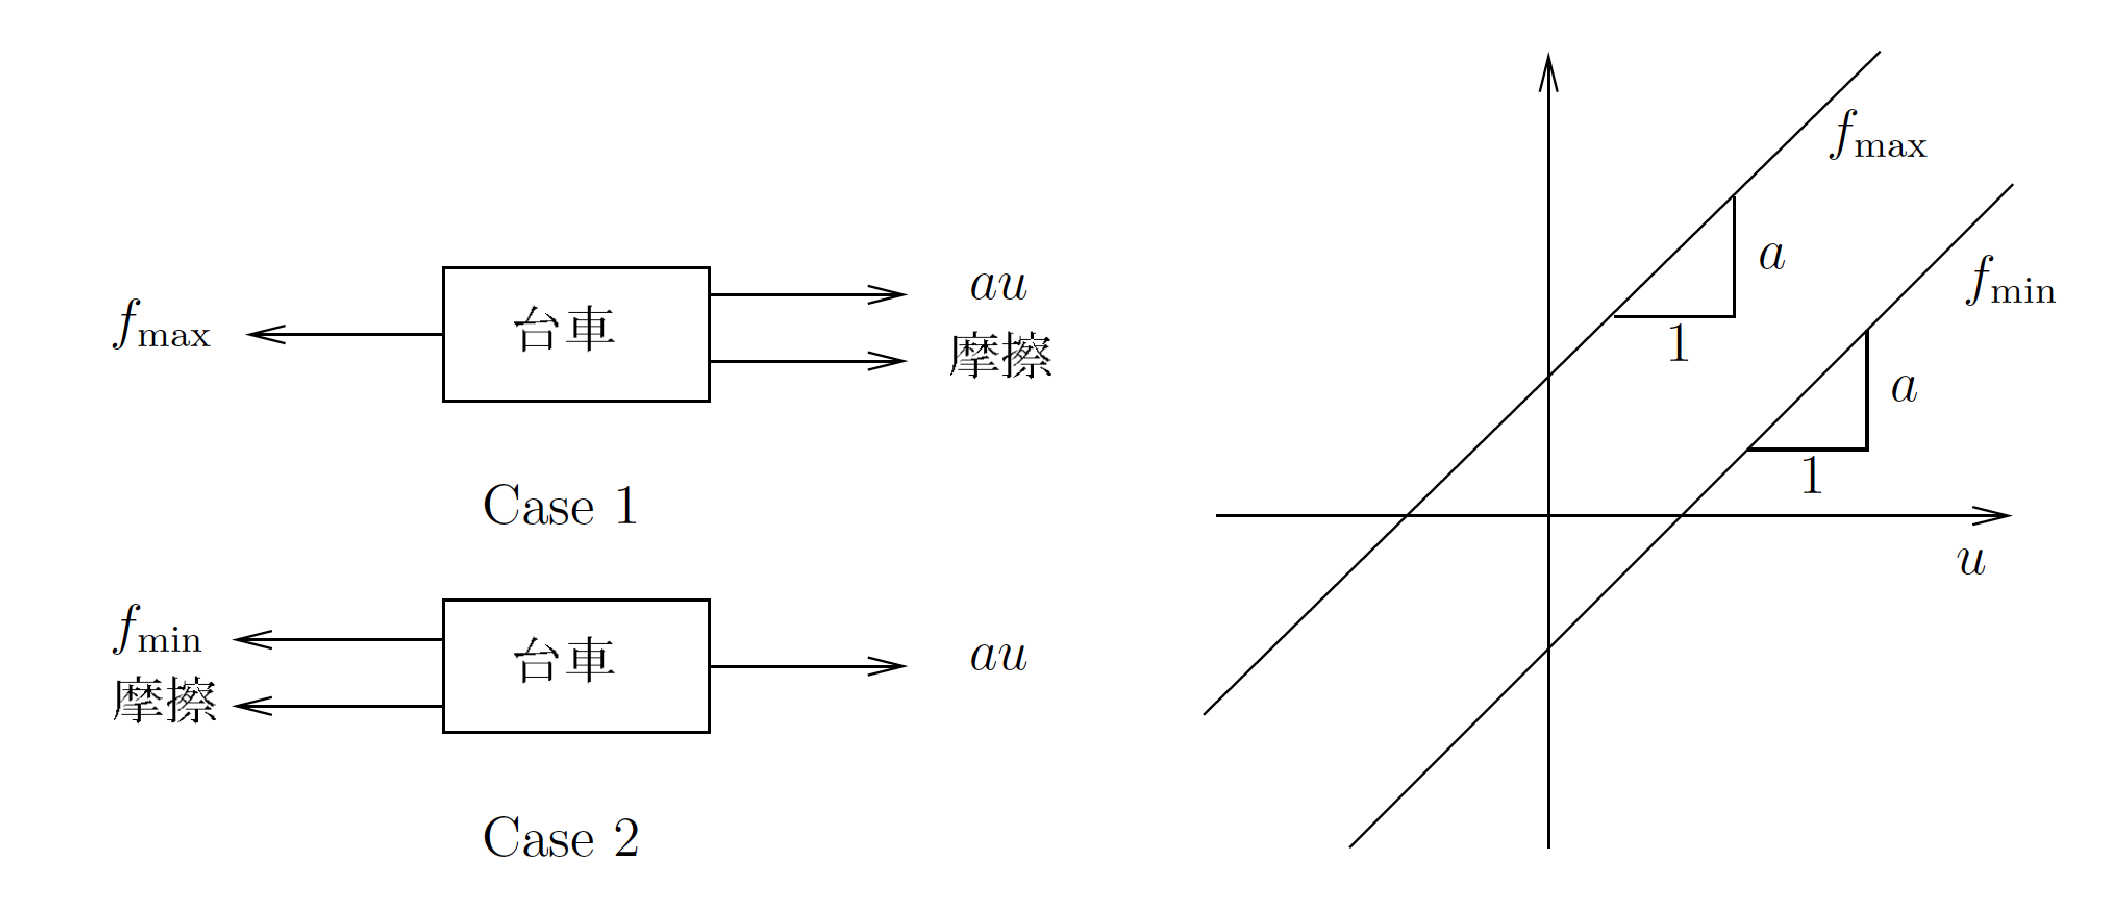
\includegraphics[width=0.6\linewidth]{definition_a.eps}
                \caption{図\ref{definition_a}: パラメータ$a$の決定}
                \label{definition_a}
            \end{center}
        \end{figure}
    \end{enumerate}

    \item 台車の変位$r$と$y_{1}$の変換係数を$c_{1} = 1.0$ [V/m], 
    振子の角度$\theta$と$y_{2}$の変換係数を$c_{2} = 1.0$ [V/rad]とする.

    \item 以下の2通りの方法で台車系の質量$M$[kg]と摩擦係数$f$[kg/s]を求める.
    \begin{itemize}
        % --- step response --- %
        \item ステップ応答による方法 \\
        \quad 振子を台車から取り外したまま,台車のステップ応答を測定する.そのとき,台車の運動方程式は,

        \begin{equation}
            M \ddot r = au - fr
            \label{eq_model}
        \end{equation}

        であり,入力$u$から目標値$r$までの伝達関数$G$は,

        \begin{equation}
            G(s) = \frac{K}{s(Ts + 1)}
        \end{equation}

        となる.ただし,

        \begin{equation}
            K = \frac{a}{f},\ T = \frac{M}{f}
        \end{equation}

        である.初期状態を零ベクトルとすれば,台車のステップ応答は,

        \begin{equation}
            r(t) = KU_{0}
            \left(
                T\exp \left(\frac{-t}{T} \right) + t - T
            \right)
            \label{step_response}
        \end{equation}

        である.(図\ref{cart_step}参照)ただし,$U_{0}$はステップ入力の$t > 0$での値である.式(\ref{step_response})
        において,$t \to \infty$の極限をとると,

        \begin{equation}
            \lim_{t \to \infty} r(t) = KU_{0}(t - T)
            \label{lim_step_response}
        \end{equation}

        となる.図\ref{cart_step}を参考に,式(\ref{lim_step_response})から$T$, $K$を求め,

        \begin{figure}[htbp]
            \begin{center}
                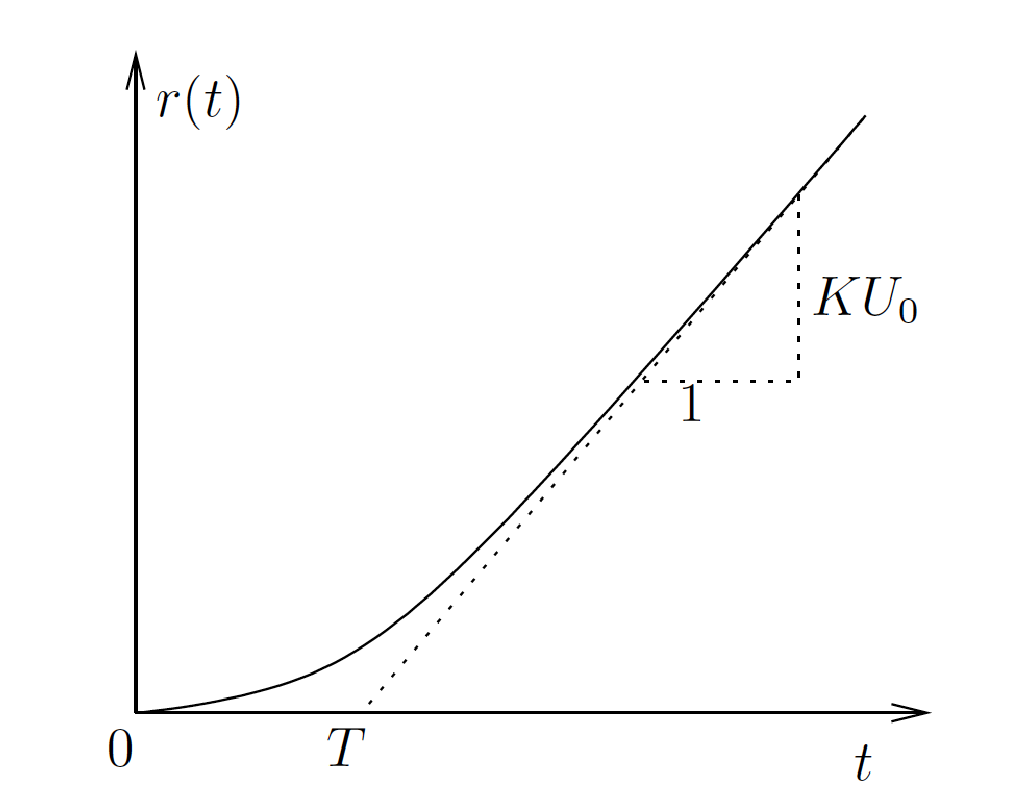
\includegraphics[width=0.6\linewidth]{cart_step.eps}
                \caption{図\ref{cart_step}: 台車のステップ応答}
                \label{cart_step}
            \end{center}
        \end{figure}

        $10$[V], $11$[V], ..., $15$[V]の各電圧をステップ入力として与え,それぞれのステップ応答
        から求めたパラメータ$T$, $K$を平均し,$M$, $f$を決定する.

        % --- feedback --- %
        \newpage
        \item フィードバックによる方法 \\
        \quad 台車の数式モデルである式(\ref{eq_model}),出力$y_{1} = c_{1}r$について,フィードバックにより
        入力を制御する.すなわち,

        \begin{equation}
            u = k(y_{c} - y_{1})
        \end{equation}

        とする($y_{c} =$ const, $k > 0$).このとき,閉ループシステムの応答は,

        \begin{equation}
            M \ddot{y_{1}} + f \dot{y_{1}} + c_{1}aky_{1} = c_{1}aky_{c}
        \end{equation}

        となる(図\ref{feedback}参照).一方,偏差$z$を加え,ばねばかりで引き,台車が正の方向に動き始めるときの力

        \begin{equation}
            z = y_{1} - y_{c}
        \end{equation}

        により定義すると,$z$は以下の式(\ref{secondary_system})に従う.

        \begin{equation}
            \ddot{z} + 2\zeta \omega_{n} \dot{z} + \omega_{n}^2 z = 0
            \label{secondary_system}
        \end{equation}

        ただし,

        \begin{equation}
            \zeta = \frac{f}{2\sqrt{c_{1}akM}},\ \omega_{n} = \sqrt{\frac{c_{1}ak}{M}}
            \label{zeta}
        \end{equation}

        である.式(\ref{secondary_system})の解は,

        $$
            0 < \zeta < 1
        $$

        のとき減衰振動となり,そのときの解は,

        $$
            z(t) = \frac{z_{0}}{\sqrt{1 - \zeta^2}} \exp(-\omega_{n} \zeta t)
            \sin{\left( \omega_{n} \sqrt{1 - \zeta^2}t + \phi \right)}
        $$

        ただし,
        
        $$
            \phi = \tan^{-1}{\frac{\sqrt{1 - \zeta^2}}{\zeta}}
        $$

        で与えられる.ここで,$z_{0} = z(0) = -y_{c}$である.いま,$T$とし,時刻$t_{1}$と$t_{2} = t_{1} + T$
        において波形$z$の山が隣り合うものとする.このとき.振幅の減衰比は,

        \begin{equation}
            \frac{|z_{2}(t_{2})|}{z_{2}(t_{1})} = \exp(-\lambda)
        \end{equation}

        となる.$\lambda$は対数減衰比であり,次が成り立つ.

        \begin{equation}
            \lambda = \frac{2\pi \zeta}{\sqrt{1 - \zeta^2}},\
            T = \frac{2\pi}{\omega_{n} \sqrt{1 - \zeta^2}}
            \label{lambda}
        \end{equation}

        従って,式(\ref{zeta}), 式(\ref{lambda})から,パラメータ$M$, $f$は,

        \begin{equation}
            M = \frac{c_{1}akT^2}{4\pi^2 + \lambda^2},\
            f = \frac{2\lambda M}{T}
        \end{equation}

        のようにして求まる.

        \begin{figure}[htbp]
            \begin{center}
                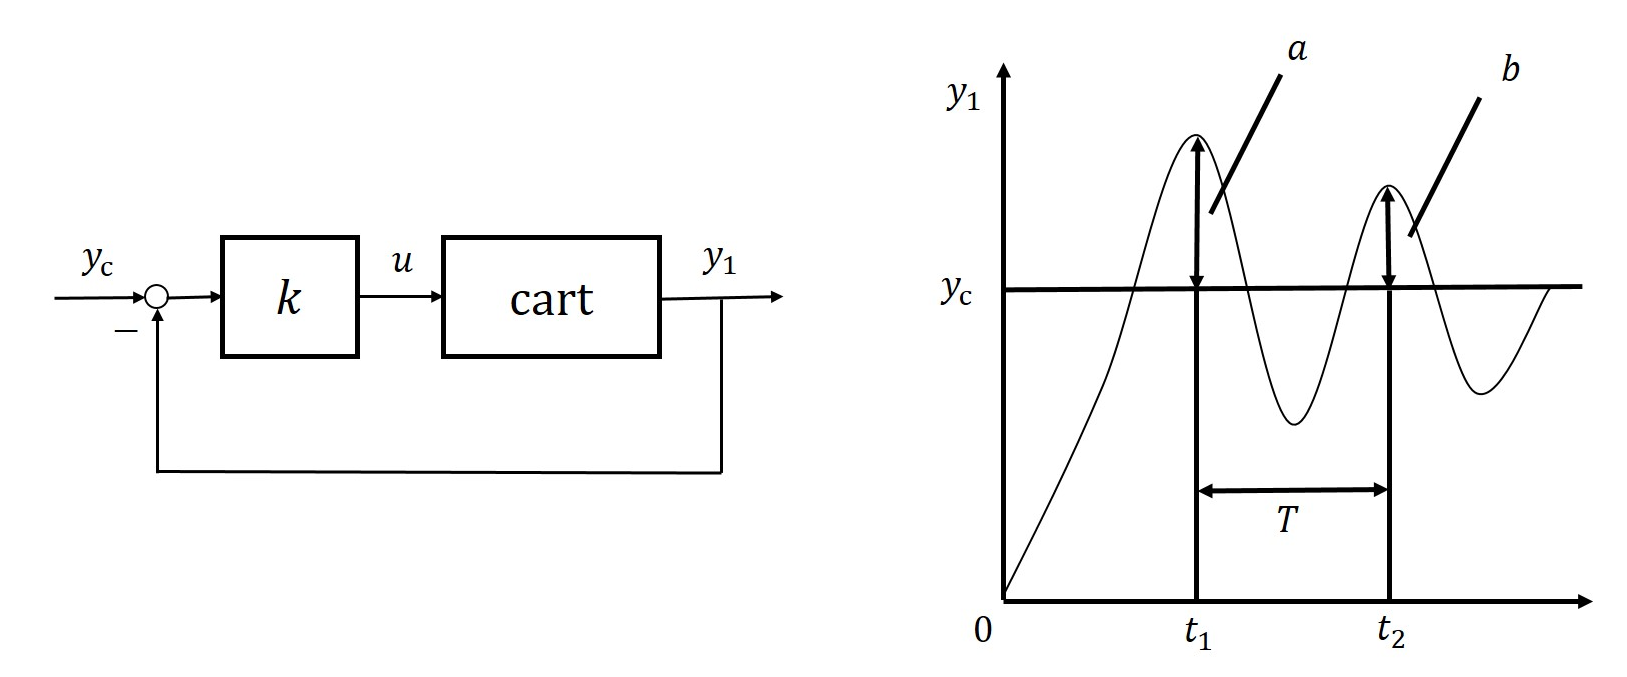
\includegraphics[width=0.6\linewidth]{feedback.eps}
                \caption{図\ref{feedback}: 台車のステップ応答}
                \label{feedback}
            \end{center}
        \end{figure}

    \end{itemize}

    \item パラメータ$J$と$c$の決定 \\
    \quad 振子を台車に取り付け,台車を固定したまま振子を自由振動させることにより,パラメータ$J$, $c$を測定する.
    このとき,振子の運動方程式は,

    \begin{equation}
        (J + ml^2) \ddot{\theta} = -mgl\sin{\theta} - c \dot{\theta}
        \label{pend_eq1}
    \end{equation}

    \begin{equation}
        y_{2} = c_{2} \theta
        \label{pend_eq2}
    \end{equation}

    で与えられる.$\theta$を微小区間で考えると,式(\ref{pend_eq1}), 式(\ref{pend_eq2})は次のように書ける.

    \begin{equation}
        \ddot{y_2} + 2\zeta \omega_{n} \dot{y_{2}} + \omega_{n}^2y_{2} = 0
        \label{pend_eq3}
    \end{equation}

    \begin{equation}
        \zeta = \frac{c}{2\sqrt{mgl(J + ml^2)}},\
        \omega_{n} = \sqrt{\frac{mgl}{J + ml^2}}
    \end{equation}

    式(\ref{pend_eq3})の解で表される減衰振動の対数減衰率を$\lambda$, 周期を$T$とすると,式(\ref{lambda})
    が成り立つことから$J$と$c$は,

    \begin{equation}
        J = \frac{mglT^2}{4\pi^2 + \lambda^2} - ml^2,\
        c = \frac{2\lambda (J + ml^2)}{T}
    \end{equation}

    のように与えられる.

\end{enumerate}


\subsection{パラメータの検証}
測定した物理パラメータを表\ref{pend_params}に示す。

\begin{table}[htbp]
    \begin{center}
        \caption{表\ref{pend_params}: 測定した物理パラメータ}
        \begin{tabular}{|l|r|} \hline
            $m$ $[\mathrm{kg}]$ & 0.038 \\ \hline
            $l$ $[\mathrm{m}]$ & 0.12 \\ \hline
            $M(\rm{Step})$ $[\mathrm{kg}]$ & 1.00 \\ \hline
            $f(\rm{Step})$ $[\mathrm{kg/s}]$ & 9.67 \\ \hline
            $M(\rm{Feedback})$ $[\mathrm{kg}]$ & 1.51 \\ \hline
            $f(\rm{Feedback})$ $[\mathrm{kg/s}]$ & 16.5 \\ \hline
            $J$ $[\mathrm{kg \cdot m^2}]$ & 3.90E-4 \\ \hline
            $c$ $[\mathrm{kg \cdot m^2/s}]$ & 9.82E-5 \\ \hline
            $a$ $[\mathrm{N/V}]$ & 0.49 \\ \hline
            $c_1$ $[\mathrm{V/m}]$ & 1.0 \\ \hline
            $c_2$ $[\mathrm{V/rad}]$ & 1.0 \\ \hline
            $g$ $[\mathrm{m/s^2}]$ & 9.8 \\ \hline
        \end{tabular}
        \label{pend_params}
    \end{center}
\end{table}

次に、表\ref{pend_params}に示すパラメータの検証を行う。

\subsection{$M$と$f$の検証}
図\ref{step13_correct}に、入力電圧$13.0$[V]のときの台車系のステップ応答とそのシミュレーションを示す。
また、図\ref{feedback_correct}に台車系のフィードバック応答とそのシミュレーションを示す。

\begin{figure}[htbp]
    \begin{center}
        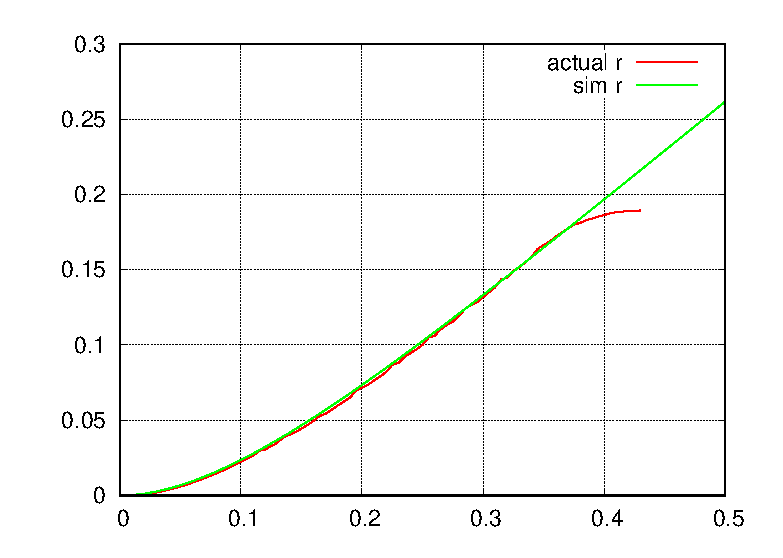
\includegraphics[width=0.6\linewidth]{step13_correct.eps}
        \caption{図\ref{step13_correct}: ステップ応答による$M$と$f$の検証}
        \label{step13_correct}
    \end{center}
\end{figure}

\begin{figure}[htbp]
    \begin{center}
        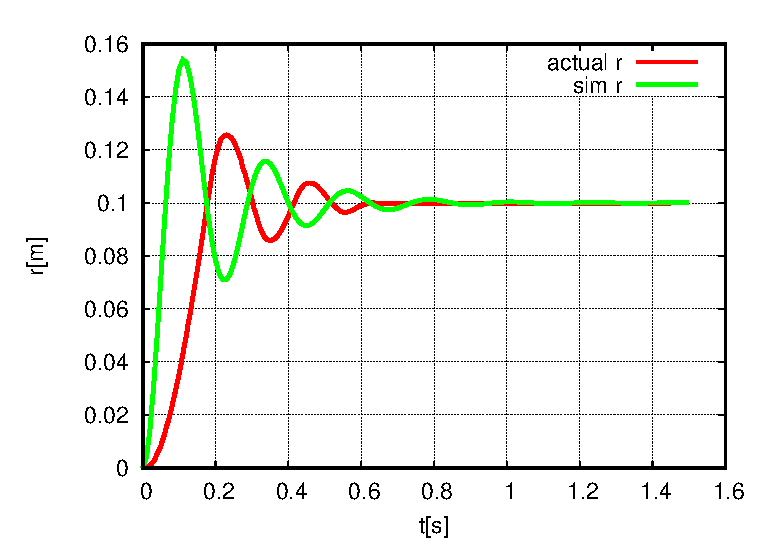
\includegraphics[width=0.6\linewidth]{feedback_correct.eps}
        \caption{図\ref{feedback_correct}: ステップ応答による$M$と$f$の検証}
        \label{feedback_correct}
    \end{center}
\end{figure}

図\ref{feedback_correct}では、シミュレーション結果と実験結果が不一致なため、不適切んばパラメータ
である。一方、図\ref{step13_correct}では、直線近似を行うために十分な一致が見られるため、
ステップ応答により測定した$M = 1.00$と$f = 9.67$を用いて実験を行う。

\subsection{$J$と$c$の検証}
図\ref{jc_correct}に振子の自由振動の応答とそのシミュレーションを示す。
実験とシミュレーションの波形を比較すると、初期位相が異なっているが、振幅と周期が近しい値をとっているので
測定した$J$ = 3.90E-4と$c$ = 9.82E-5を実験に用いる。

\begin{figure}[htbp]
    \begin{center}
        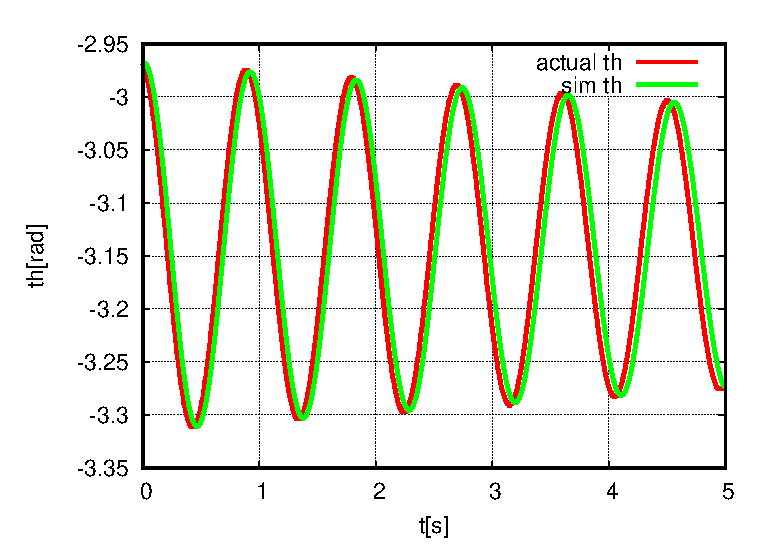
\includegraphics[width=0.6\linewidth]{jc_correct.eps}
        \caption{図\ref{jc_correct}: 自由振動による$J$と$c$の検証}
        \label{jc_correct}
    \end{center}
\end{figure}



% =============================== chapter 2 END =============================== %